% Options for packages loaded elsewhere
\PassOptionsToPackage{unicode}{hyperref}
\PassOptionsToPackage{hyphens}{url}
%
\documentclass[
]{article}
\usepackage{amsmath,amssymb}
\usepackage{lmodern}
\usepackage{iftex}
\ifPDFTeX
  \usepackage[T1]{fontenc}
  \usepackage[utf8]{inputenc}
  \usepackage{textcomp} % provide euro and other symbols
\else % if luatex or xetex
  \usepackage{unicode-math}
  \defaultfontfeatures{Scale=MatchLowercase}
  \defaultfontfeatures[\rmfamily]{Ligatures=TeX,Scale=1}
\fi
% Use upquote if available, for straight quotes in verbatim environments
\IfFileExists{upquote.sty}{\usepackage{upquote}}{}
\IfFileExists{microtype.sty}{% use microtype if available
  \usepackage[]{microtype}
  \UseMicrotypeSet[protrusion]{basicmath} % disable protrusion for tt fonts
}{}
\makeatletter
\@ifundefined{KOMAClassName}{% if non-KOMA class
  \IfFileExists{parskip.sty}{%
    \usepackage{parskip}
  }{% else
    \setlength{\parindent}{0pt}
    \setlength{\parskip}{6pt plus 2pt minus 1pt}}
}{% if KOMA class
  \KOMAoptions{parskip=half}}
\makeatother
\usepackage{xcolor}
\usepackage[margin=1in]{geometry}
\usepackage{longtable,booktabs,array}
\usepackage{calc} % for calculating minipage widths
% Correct order of tables after \paragraph or \subparagraph
\usepackage{etoolbox}
\makeatletter
\patchcmd\longtable{\par}{\if@noskipsec\mbox{}\fi\par}{}{}
\makeatother
% Allow footnotes in longtable head/foot
\IfFileExists{footnotehyper.sty}{\usepackage{footnotehyper}}{\usepackage{footnote}}
\makesavenoteenv{longtable}
\usepackage{graphicx}
\makeatletter
\def\maxwidth{\ifdim\Gin@nat@width>\linewidth\linewidth\else\Gin@nat@width\fi}
\def\maxheight{\ifdim\Gin@nat@height>\textheight\textheight\else\Gin@nat@height\fi}
\makeatother
% Scale images if necessary, so that they will not overflow the page
% margins by default, and it is still possible to overwrite the defaults
% using explicit options in \includegraphics[width, height, ...]{}
\setkeys{Gin}{width=\maxwidth,height=\maxheight,keepaspectratio}
% Set default figure placement to htbp
\makeatletter
\def\fps@figure{htbp}
\makeatother
\setlength{\emergencystretch}{3em} % prevent overfull lines
\providecommand{\tightlist}{%
  \setlength{\itemsep}{0pt}\setlength{\parskip}{0pt}}
\setcounter{secnumdepth}{5}
\newlength{\cslhangindent}
\setlength{\cslhangindent}{1.5em}
\newlength{\csllabelwidth}
\setlength{\csllabelwidth}{3em}
\newlength{\cslentryspacingunit} % times entry-spacing
\setlength{\cslentryspacingunit}{\parskip}
\newenvironment{CSLReferences}[2] % #1 hanging-ident, #2 entry spacing
 {% don't indent paragraphs
  \setlength{\parindent}{0pt}
  % turn on hanging indent if param 1 is 1
  \ifodd #1
  \let\oldpar\par
  \def\par{\hangindent=\cslhangindent\oldpar}
  \fi
  % set entry spacing
  \setlength{\parskip}{#2\cslentryspacingunit}
 }%
 {}
\usepackage{calc}
\newcommand{\CSLBlock}[1]{#1\hfill\break}
\newcommand{\CSLLeftMargin}[1]{\parbox[t]{\csllabelwidth}{#1}}
\newcommand{\CSLRightInline}[1]{\parbox[t]{\linewidth - \csllabelwidth}{#1}\break}
\newcommand{\CSLIndent}[1]{\hspace{\cslhangindent}#1}
\newcommand{\beginappendix}{ \setcounter{table}{0} \renewcommand{\thetable}{A\arabic{table}} \setcounter{figure}{0} \renewcommand{\thefigure}{A\arabic{figure}} }
\usepackage[capposition=top]{floatrow}
\usepackage{placeins}
\usepackage{setspace}
\usepackage{dcolumn}
\usepackage{booktabs}
\usepackage{siunitx}
\usepackage{amsmath}
\usepackage{enumerate}
\usepackage[shortlabels]{enumitem}
\usepackage[hang,flushmargin]{footmisc}
\usepackage{booktabs}
\usepackage{longtable}
\usepackage{array}
\usepackage{multirow}
\usepackage{wrapfig}
\usepackage{float}
\usepackage{colortbl}
\usepackage{pdflscape}
\usepackage{tabu}
\usepackage{threeparttable}
\usepackage{threeparttablex}
\usepackage[normalem]{ulem}
\usepackage{makecell}
\usepackage{xcolor}
\ifLuaTeX
  \usepackage{selnolig}  % disable illegal ligatures
\fi
\IfFileExists{bookmark.sty}{\usepackage{bookmark}}{\usepackage{hyperref}}
\IfFileExists{xurl.sty}{\usepackage{xurl}}{} % add URL line breaks if available
\urlstyle{same} % disable monospaced font for URLs
\hypersetup{
  pdftitle={Pollution, agricultural productivity, and development: Evidence from coal in plants in India},
  pdfauthor={Joshua D. Merfeld},
  hidelinks,
  pdfcreator={LaTeX via pandoc}}

\title{Pollution, agricultural productivity, and development: Evidence from coal in plants in India\footnote{thanks to\ldots{}}}
\author{Joshua D. Merfeld\footnote{KDI School of Public Policy and Management and IZA; \href{mailto:merfeld@kdis.ac.kr}{\nolinkurl{merfeld@kdis.ac.kr}}}}
\date{2023-01-03}

\begin{document}
\maketitle
\begin{abstract}
\noindent abstract\\
\strut \\
\textbf{\textit{Keywords}}:\\
\textbf{\textit{JEL Codes}}:
\end{abstract}

\newpage
\doublespacing

\hypertarget{introduction}{%
\section{Introduction}\label{introduction}}

pollution could be bad for agriculture Marshall et al. (1997)

lower agricultural productivity near gold mines in Ghana (Aragón and Rud 2016); apparently lots of pollution
- ``The main identification assumption is that the change in agricultural productivity over time in both areas would be similar in the absence of mining.''
- within 20km
- also finds suggestive evidence it's not all labor productivity changes

``Much of what we know about the marginal effect of pollution on infant mortality is derived from developed country data. However, given the lower levels of air pollution in developed countries, these estimates may not be externally valid to the developing country context if there is a non-linear dose relationship between pollution and mortality or if the costs of avoidance behaviour differ considerably between the two contexts. In this article, we estimate the relationship between pollution and infant mortality using data from Mexico. Our estimates for PM10 tend to be similar (or even smaller) than the US estimates, while our findings on CO tend to be larger than those derived from the US context.'' (Arceo, Hanna, and Oliva 2016)

We have known about the effects of pollution on human health for many years Pope III and Dockery (2006)
good review on the effects of pollution early in life in Currie et al. (2014)
- also in developing countries, where there is a consistent effect of exposure on infant mortality (Heft-Neal et al. 2018)

``Air pollution has both acute and chronic effects on human health, affecting a number of different systems and organs. It ranges from minor upper respiratory irritation to chronic respiratory and heart disease, lung cancer, acute respiratory infections in children and chronic bronchitis in adults, aggravating pre-existing heart and lung disease, or asthmatic attacks. In addition, short- and long-term exposures have also been linked with premature mortality and reduced life expectancy. These effects of air pollutants on human health and their mechanism of action are briefly discussed.'' Kampa and Castanas (2008)

worker productivity and cognitive function:
- call center workers in China, and at common levels of pollution (Chang et al. 2019)
- tests (Ebenstein, Lavy, and Roth 2016)
- farm workers in California (Graff Zivin and Neidell 2012)
- increase in extensive margin (Hanna and Oliva 2015)
- manufacturing in China (He, Liu, and Salvo 2019); ``We uncover statistically significant adverse output effects from more prolonged exposure, but effects are not large. A substantial +10 mug/m3 PM2.5 variation sustained over 25 days reduces daily output by 1 percent.''

induces migration (Chen, Oliva, and Zhang 2022)

overall effects on agricultural productivity taking into accounts any changes in input allocation caused by the increase in pollution.

\hypertarget{data-and-methods}{%
\section{Data and methods}\label{data-and-methods}}

\hypertarget{data}{%
\subsection{Data}\label{data}}

Asher et al. (2021)
Ag productivity: Gangopadhyay et al. (2022)
PM estimates: Hammer et al. (2020)

\begin{table}

\caption{\label{tab:data}Remote sensing data sources}
\centering
\begin{threeparttable}
\begin{tabular}[t]{>{\raggedright\arraybackslash}p{3cm}>{\centering\arraybackslash}p{2cm}>{\centering\arraybackslash}p{2cm}>{\centering\arraybackslash}p{2cm}>{\centering\arraybackslash}p{2cm}>{\centering\arraybackslash}p{2cm}}
\toprule
  & shapefile & wind & pollution & agriculture & nightlights\\
\midrule
source & Asher et al. (2021) & NCAR & Hammer et al. (2020) & Angopadhyay et al. (2022) & Asher et al. (2021)\\
geographic coverage & India & global & global & global & India\\
temporal coverage &  & daily & monthly & two seasons/year & yearly\\
\bottomrule
\end{tabular}
\begin{tablenotes}
\item \textit{ } 
\item NCAR: https://climatedataguide.ucar.edu/
\end{tablenotes}
\end{threeparttable}
\end{table}

\hypertarget{methodology}{%
\subsection{Methodology}\label{methodology}}

\begin{figure}
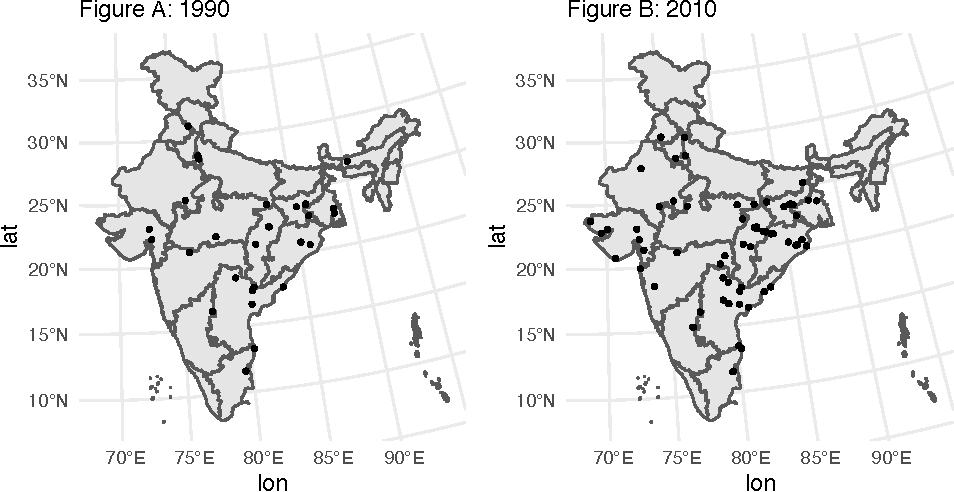
\includegraphics{draft_files/figure-latex/plants-1} \caption[Coal plants in India from 1990 to 2010]{Coal plants in India from 1990 to 2010}\label{fig:plants}\floatfoot*{Note: The top figure shows the location of coal plants in 1990. The bottom figure shows the location of coal plants in 2010.}
\end{figure}

\begin{figure}
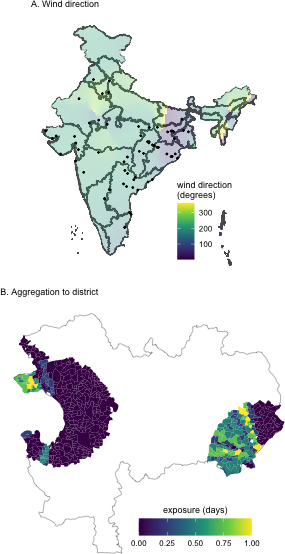
\includegraphics{draft_files/figure-latex/windexample-1} \caption[Wind direction and aggregation examples (2010-01-01)]{Wind direction and aggregation examples (2010-01-01)}\label{fig:windexample}\floatfoot*{Note: The top figure shows the average wind direction on January 1st, 2010. The points are the location of coal plants on that date. The bottom figure shows the distribution of pollution exposure in a specific district -- Kangra district in Himachal Pradesh -- on the same date.}
\end{figure}

\newpage

\begin{table}

\caption{\label{tab:pollutiontable}Wind direction and particulate matter}
\centering
\begin{threeparttable}
\begin{tabular}[t]{>{\raggedright\arraybackslash}p{4cm}>{\centering\arraybackslash}p{2cm}>{\centering\arraybackslash}p{2cm}>{\centering\arraybackslash}p{2cm}>{\centering\arraybackslash}p{2cm}}
\toprule
\multicolumn{1}{c}{ } & \multicolumn{2}{c}{1998-2015} & \multicolumn{2}{c}{2002-2013} \\
\cmidrule(l{3pt}r{3pt}){2-3} \cmidrule(l{3pt}r{3pt}){4-5}
  & (1) & (2) & (3) & (4)\\
\midrule
wind & 0.045*** & 0.014*** & 0.063*** & 0.015***\\
 & (0.004) & (0.001) & (0.005) & (0.002)\\
\textbf{fixed effects:} & \textbf{} & \textbf{} & \textbf{} & \textbf{}\\
village & Yes & Yes & Yes & Yes\\
month & Yes & No & Yes & No\\
district-month & No & Yes & No & Yes\\
\midrule
observations & 22,345,092 & 22,345,092 & 14,896,728 & 14,896,728\\
\bottomrule
\end{tabular}
\begin{tablenotes}
\item Note: Standard errors are in parentheses and are clustered at the village level.
\item * p<0.10 ** p<0.05 *** p<0.01
\end{tablenotes}
\end{threeparttable}
\end{table}

\hypertarget{results}{%
\section{Results}\label{results}}

\begin{table}

\caption{\label{tab:yieldtable}Wind direction and agricultural productivity}
\centering
\begin{threeparttable}
\begin{tabular}[t]{>{\raggedright\arraybackslash}p{3cm}>{\centering\arraybackslash}p{2cm}>{\centering\arraybackslash}p{2cm}>{\centering\arraybackslash}p{2cm}>{\centering\arraybackslash}p{2cm}>{\centering\arraybackslash}p{2cm}}
\toprule
\multicolumn{1}{c}{ } & \multicolumn{3}{c}{all} & \multicolumn{1}{c}{monsoon} & \multicolumn{1}{c}{winter} \\
\cmidrule(l{3pt}r{3pt}){2-4} \cmidrule(l{3pt}r{3pt}){5-5} \cmidrule(l{3pt}r{3pt}){6-6}
  & (1) & (2) & (3) & (4) & (5)\\
\midrule
wind & -0.003*** & -0.003*** & -0.0007*** & -0.002*** & -0.003***\\
 & (0.0002) & (0.0002) & (9.21e-5) & (0.0002) & (0.0003)\\
rain (z) &  & 0.029*** & 0.009*** & 0.082*** & 0.016***\\
 &  & (0.0004) & (0.001) & (0.002) & (0.0004)\\
\textbf{fixed effects:} & \textbf{} & \textbf{} & \textbf{} & \textbf{} & \textbf{}\\
village-season & Yes & Yes & Yes & No & No\\
year & Yes & Yes & No & Yes & Yes\\
district-year-season & No & No & Yes & No & No\\
village & No & No & No & Yes & Yes\\
\midrule
observations & 2,391,533 & 2,375,337 & 2,375,337 & 1,259,123 & 1,116,214\\
\bottomrule
\end{tabular}
\begin{tablenotes}
\item Note: Standard errors are in parentheses and are clustered at the village level.
\item * p<0.10 ** p<0.05 *** p<0.01
\end{tablenotes}
\end{threeparttable}
\end{table}

\begin{table}

\caption{\label{tab:yieldtabletwo}Pollution and agricultural productivity, IV estimates}
\centering
\begin{threeparttable}
\begin{tabular}[t]{>{\raggedright\arraybackslash}p{3.5cm}>{\centering\arraybackslash}p{2cm}>{\centering\arraybackslash}p{2cm}>{\centering\arraybackslash}p{2cm}>{\centering\arraybackslash}p{2cm}>{\centering\arraybackslash}p{2cm}}
\toprule
\multicolumn{1}{c}{ } & \multicolumn{3}{c}{all} & \multicolumn{1}{c}{monsoon} & \multicolumn{1}{c}{winter} \\
\cmidrule(l{3pt}r{3pt}){2-4} \cmidrule(l{3pt}r{3pt}){5-5} \cmidrule(l{3pt}r{3pt}){6-6}
  & (1) & (2) & (3) & (4) & (5)\\
\midrule
particulate matter & -0.021*** & -0.020*** & -0.033*** & -0.013*** & -0.024***\\
(PM 2.5, '000s) & (0.001) & (0.002) & (0.005) & (0.001) & (0.003)\\
rain (z) &  & 0.004** & 0.002 & 0.086*** & -0.016***\\
 &  & (0.002) & (0.002) & (0.002) & (0.004)\\
\textbf{fixed effects:} & \textbf{} & \textbf{} & \textbf{} & \textbf{} & \textbf{}\\
village-season & Yes & Yes & Yes & No & No\\
year & Yes & Yes & No & Yes & Yes\\
district-year-season & No & No & Yes & No & No\\
village & No & No & No & Yes & Yes\\
\midrule
observations & 2,391,533 & 2,375,337 & 2,375,337 & 1,259,123 & 1,116,214\\
\midrule
first stage: &  &  &  &  & \\
wind & 0.143*** & 0.126*** & 0.022*** & 0.155*** & 0.105***\\
 & (0.003) & (0.003) & (0.002) & (0.003) & (0.004)\\
rain (z) &  & -1.23*** & -0.235*** & 0.301*** & -1.36***\\
 &  & (0.010) & (0.018) & (0.015) & (0.009)\\
\bottomrule
\end{tabular}
\begin{tablenotes}
\item Note: Standard errors are in parentheses and are clustered at the village level.
\item * p<0.10 ** p<0.05 *** p<0.01
\end{tablenotes}
\end{threeparttable}
\end{table}

\begin{table}

\caption{\label{tab:yieldtablehet}Heterogeneity in the effects of pollution on productivity}
\centering
\begin{threeparttable}
\begin{tabular}[t]{>{\raggedright\arraybackslash}p{4cm}>{\centering\arraybackslash}p{2cm}>{\centering\arraybackslash}p{2cm}>{\centering\arraybackslash}p{2cm}>{\centering\arraybackslash}p{2cm}>{\centering\arraybackslash}p{2cm}}
\toprule
\multicolumn{1}{c}{ } & \multicolumn{1}{c}{>p(50)} & \multicolumn{1}{c}{<=p(50)} & \multicolumn{3}{c}{all} \\
\cmidrule(l{3pt}r{3pt}){2-2} \cmidrule(l{3pt}r{3pt}){3-3} \cmidrule(l{3pt}r{3pt}){4-6}
  & (1) & (2) & (3) & (4) & (5\\
\midrule
wind & -0.003*** & -0.032*** & -0.004*** & 0.0004 & -0.0001\\
 & (0.0002) & (0.002) & (0.0003) & (0.0005) & (0.001)\\
rain (z) & 0.031*** & 0.030*** & 0.029*** & 0.029*** & 0.029***\\
 & (0.0006) & (0.0005) & (0.0004) & (0.0004) & (0.0004)\\
wind x rain &  &  & 0.0005*** &  & \\
 &  &  & (6.67e-5) &  & \\
wind squared &  &  &  & -0.0002*** & \\
 &  &  &  & (3.54e-5) & \\
wind x starting yield &  &  &  &  & -0.001**\\
 &  &  &  &  & (0.0006)\\
\textbf{fixed effects:} & \textbf{} & \textbf{} & \textbf{} & \textbf{} & \textbf{}\\
village-season & Yes & Yes & Yes & Yes & Yes\\
year & Yes & Yes & Yes & Yes & Yes\\
\midrule
observations & 1,115,694 & 1,259,643 & 2,375,337 & 2,375,337 & 2,371,364\\
\bottomrule
\end{tabular}
\begin{tablenotes}
\item Note: Standard errors are in parentheses and are clustered at the village level.
\item * p<0.10 ** p<0.05 *** p<0.01
\end{tablenotes}
\end{threeparttable}
\end{table}

\begin{table}

\caption{\label{tab:labortable}Wind direction and labor allocation}
\centering
\begin{threeparttable}
\begin{tabular}[t]{>{\raggedright\arraybackslash}p{3cm}>{\centering\arraybackslash}p{1.5cm}>{\centering\arraybackslash}p{1.5cm}>{\centering\arraybackslash}p{1.5cm}>{\centering\arraybackslash}p{1.5cm}>{\centering\arraybackslash}p{1.5cm}>{\centering\arraybackslash}p{1.5cm}}
\toprule
  & all & all & self & wage & farm & non-farm\\
\midrule
wind & -0.021 & -0.027* & 0.008 & -0.034** & 0.035* & -0.061**\\
 & (0.015) & (0.015) & (0.017) & (0.016) & (0.019) & (0.025)\\
controls & No & Yes & Yes & Yes & Yes & Yes\\
\textbf{fixed effects:} & \textbf{} & \textbf{} & \textbf{} & \textbf{} & \textbf{} & \textbf{}\\
district & Yes & Yes & Yes & Yes & Yes & Yes\\
year & Yes & Yes & Yes & Yes & Yes & Yes\\
\textbf{varying slopes:} & \textbf{} & \textbf{} & \textbf{} & \textbf{} & \textbf{} & \textbf{}\\
year (by district) & Yes & Yes & Yes & Yes & Yes & Yes\\
\midrule
observations & 899,045 & 898,856 & 898,856 & 898,856 & 898,856 & 898,856\\
\bottomrule
\end{tabular}
\begin{tablenotes}
\item Note: Standard errors are in parentheses and are clustered at the district level. Control variables include female, age, age squared, and (years of) education.
\item * p<0.10 ** p<0.05 *** p<0.01
\end{tablenotes}
\end{threeparttable}
\end{table}

\begin{table}

\caption{\label{tab:ntltable}Wind direction and nightlight growth}
\centering
\begin{threeparttable}
\begin{tabular}[t]{>{\raggedright\arraybackslash}p{3cm}>{\centering\arraybackslash}p{2cm}>{\centering\arraybackslash}p{2cm}}
\toprule
  & (1) & (2)\\
\midrule
wind (lagged) & -0.080*** & -0.083***\\
 & (0.015) & (0.015)\\
rain (z, lagged) &  & -0.035***\\
 &  & (0.002)\\
\textbf{fixed effects:} & \textbf{} & \textbf{}\\
village & Yes & Yes\\
year & Yes & Yes\\
\textbf{varying slopes:} & \textbf{} & \textbf{}\\
year (by village) & Yes & Yes\\
\midrule
observations & 2,146,715 & 2,146,715\\
\bottomrule
\end{tabular}
\begin{tablenotes}
\item Note: Standard errors are in parentheses and are clustered at the village level.
\item * p<0.10 ** p<0.05 *** p<0.01
\end{tablenotes}
\end{threeparttable}
\end{table}

\hypertarget{conclusion}{%
\section{Conclusion}\label{conclusion}}

\FloatBarrier
\newpage

\newpage
\singlespacing

\hypertarget{references}{%
\section*{References}\label{references}}
\addcontentsline{toc}{section}{References}

\hypertarget{refs}{}
\begin{CSLReferences}{1}{0}
\leavevmode\vadjust pre{\hypertarget{ref-aragon2016polluting}{}}%
Aragón, Fernando M, and Juan Pablo Rud. 2016. {``{Polluting industries and agricultural productivity: Evidence from mining in Ghana}.''} \emph{{The Economic Journal}} 126 (597): 1980--2011.

\leavevmode\vadjust pre{\hypertarget{ref-arceo2016does}{}}%
Arceo, Eva, Rema Hanna, and Paulina Oliva. 2016. {``{Does the effect of pollution on infant mortality differ between developing and developed countries? Evidence from Mexico City}.''} \emph{{The Economic Journal}} 126 (591): 257--80.

\leavevmode\vadjust pre{\hypertarget{ref-almn2021}{}}%
Asher, Sam, Tobias Lunt, Ryu Matsuura, and Paul Novosad. 2021. {``{Development Research at High Geographic Resolution: An Analysis of Night Lights, Firms, and Poverty in India using the SHRUG Open Data Platform}.''} \emph{{The World Bank Economic Review}}.

\leavevmode\vadjust pre{\hypertarget{ref-brunekreef2002air}{}}%
Brunekreef, Bert, and Stephen T Holgate. 2002. {``{Air pollution and health}.''} \emph{{The Lancet}} 360 (9341): 1233--42.

\leavevmode\vadjust pre{\hypertarget{ref-chang2019effect}{}}%
Chang, Tom Y, Joshua Graff Zivin, Tal Gross, and Matthew Neidell. 2019. {``{The effect of pollution on worker productivity: evidence from call center workers in China}.''} \emph{{American Economic Journal: Applied Economics}} 11 (1): 151--72.

\leavevmode\vadjust pre{\hypertarget{ref-chen2022effect}{}}%
Chen, Shuai, Paulina Oliva, and Peng Zhang. 2022. {``{The effect of air pollution on migration: evidence from China}.''} \emph{{Journal of Development Economics}} 156: 102833.

\leavevmode\vadjust pre{\hypertarget{ref-currie2014we}{}}%
Currie, Janet, Joshua Graff Zivin, Jamie Mullins, and Matthew Neidell. 2014. {``{What do we know about short-and long-term effects of early-life exposure to pollution?}''} \emph{{Annual Review Resource Economics}} 6 (1): 217--47.

\leavevmode\vadjust pre{\hypertarget{ref-ebenstein2016long}{}}%
Ebenstein, Avraham, Victor Lavy, and Sefi Roth. 2016. {``{The long-run economic consequences of high-stakes examinations: Evidence from transitory variation in pollution}.''} \emph{{American Economic Journal: Applied Economics}} 8 (4): 36--65.

\leavevmode\vadjust pre{\hypertarget{ref-gangopadhyay2022new}{}}%
Gangopadhyay, Prasun K, Paresh B Shirsath, Vinay K Dadhwal, and Pramod K Aggarwal. 2022. {``{A new two-decade (2001--2019) high-resolution agricultural primary productivity dataset for India}.''} \emph{{Scientific Data}} 9 (1): 1--12.

\leavevmode\vadjust pre{\hypertarget{ref-graff2012impact}{}}%
Graff Zivin, Joshua, and Matthew Neidell. 2012. {``{The impact of pollution on worker productivity}.''} \emph{{American Economic Review}} 102 (7): 3652--73.

\leavevmode\vadjust pre{\hypertarget{ref-hammer2020global}{}}%
Hammer, Melanie S, Aaron van Donkelaar, Chi Li, Alexei Lyapustin, Andrew M Sayer, N Christina Hsu, Robert C Levy, et al. 2020. {``Global Estimates and Long-Term Trends of Fine Particulate Matter Concentrations (1998--2018).''} \emph{{Environmental Science \& Technology}} 54 (13): 7879--90.

\leavevmode\vadjust pre{\hypertarget{ref-hanna2015effect}{}}%
Hanna, Rema, and Paulina Oliva. 2015. {``{The effect of pollution on labor supply: Evidence from a natural experiment in Mexico City}.''} \emph{{Journal of Public Economics}} 122: 68--79.

\leavevmode\vadjust pre{\hypertarget{ref-he2019severe}{}}%
He, Jiaxiu, Haoming Liu, and Alberto Salvo. 2019. {``{Severe air pollution and labor productivity: Evidence from industrial towns in China}.''} \emph{{American Economic Journal: Applied Economics}} 11 (1): 173--201.

\leavevmode\vadjust pre{\hypertarget{ref-heck1982assessment}{}}%
Heck, Walter W, OC Taylor, Richard Adams, Gail Bingham, Joseph Miller, Eric Preston, and Leonard Weinstein. 1982. {``{Assessment of crop loss from ozone}.''} \emph{{Journal of the Air Pollution Control Association}} 32 (4): 353--61.

\leavevmode\vadjust pre{\hypertarget{ref-heft2018robust}{}}%
Heft-Neal, Sam, Jennifer Burney, Eran Bendavid, and Marshall Burke. 2018. {``{Robust relationship between air quality and infant mortality in Africa}.''} \emph{Nature} 559 (7713): 254--58.

\leavevmode\vadjust pre{\hypertarget{ref-kampa2008human}{}}%
Kampa, Marilena, and Elias Castanas. 2008. {``{Human health effects of air pollution}.''} \emph{{Environmental Pollution}} 151 (2): 362--67.

\leavevmode\vadjust pre{\hypertarget{ref-marshall1997hidden}{}}%
Marshall, Fiona, Mike Ashmore, Fiona Hinchcliffe, et al. 1997. \emph{{A hidden threat to food production: Air pollution and agriculture in the developing world}}. {International Institute for Environment and Development.}

\leavevmode\vadjust pre{\hypertarget{ref-pope2006health}{}}%
Pope III, C Arden, and Douglas W Dockery. 2006. {``{Health effects of fine particulate air pollution: lines that connect}.''} \emph{{Journal of the Air \& Waste Management Association}} 56 (6): 709--42.

\end{CSLReferences}

\FloatBarrier

\beginappendix

\newpage

\hypertarget{appendix-a}{%
\section*{Appendix A}\label{appendix-a}}
\addcontentsline{toc}{section}{Appendix A}

\begin{table}

\caption{\label{tab:yieldtableleads}Agricultural productivity and pollution leads}
\centering
\begin{threeparttable}
\begin{tabular}[t]{>{\raggedright\arraybackslash}p{3cm}>{\centering\arraybackslash}p{2cm}>{\centering\arraybackslash}p{2cm}}
\toprule
  & (1) & (2)\\
\midrule
wind (lag) & 0.004*** & 0.0006*\\
 & (0.0007) & (0.0003)\\
wind & -0.002*** & -0.0007***\\
 & (0.0004) & (0.0002)\\
wind (lead) & -0.004*** & -0.0001\\
 & (0.0001) & (9.8e-5)\\
rain (z) & 0.021*** & 0.008***\\
 & (0.0005) & (0.001)\\
\textbf{fixed effects:} & \textbf{} & \textbf{}\\
village-season & Yes & Yes\\
year & Yes & No\\
district-year-season & No & Yes\\
\midrule
observations & 1,979,635 & 1,979,635\\
\bottomrule
\end{tabular}
\begin{tablenotes}
\item Note: Standard errors are in parentheses and are clustered at the village level.
\item * p<0.10 ** p<0.05 *** p<0.01
\end{tablenotes}
\end{threeparttable}
\end{table}

\end{document}
